\documentclass[14pt]{extarticle}
\usepackage[utf8]{inputenc}
\usepackage[T1]{fontenc}
\usepackage[spanish,es-lcroman]{babel}
\usepackage{amsmath}
\usepackage{amsthm}
\usepackage{physics}
\usepackage{tikz}
\usepackage{float}
\usepackage[autostyle,spanish=mexican]{csquotes}
\usepackage[per-mode=symbol]{siunitx}
\usepackage{gensymb}
\usepackage{multicol}
\usepackage{enumitem}
\usepackage{circuitikz}
\usepackage[left=2.00cm, right=2.00cm, top=2.00cm, 
     bottom=2.00cm]{geometry}
\usepackage{makecell}

\newcommand{\textocolor}[2]{\textbf{\textcolor{#1}{#2}}}
\sisetup{per-mode=symbol}
\DeclareSIUnit[number-unit-product = {\,}]\cal{cal}
\DeclareSIUnit{\dB}{dB}
%\renewcommand{\questionlabel}{\thequestion)}
\decimalpoint
\sisetup{bracket-numbers = false}

\title{\vspace*{-2cm} Ejercicios Electricidad - Solución \vspace{-5ex}}
\date{}

\begin{document}
\maketitle

\begin{enumerate}
\item Cierto foco tiene una resistencia de \SI{240}{\ohm} cuando se enciende. ¿Cuánta corriente fluirá a través del foco cuando se conecta a \SI{120}{\volt}? que es su voltaje de operación normal.

\textbf{Datos: } $R = \SI{240}{\ohm}, \quad \quad V = \SI{120}{\volt}, \quad \quad I = \, ?$

\textbf{Expresión: } $V = I \, R \hspace{0.5cm} \Rightarrow \hspace{0.5cm} I = \dfrac{V}{R}$

\textbf{Sustitución: }
\begin{align*}
I = \dfrac{V}{I} = \dfrac{\SI{120}{\volt}}{\SI{240}{\ohm}} = \SI{0.5}{\ampere}
\end{align*}
\item Un calentador eléctrico utiliza \SI{5.0}{\ampere} cuando se conecta a \SI{110}{\volt}. Determina su resistencia.

\textbf{Datos: } $I = \SI{5.0}{\ampere}, \quad \quad V = \SI{110}{\volt}, \quad \quad I = \, ?$

\textbf{Expresión: } $V = I \, R \hspace{0.5cm} \Rightarrow \hspace{0.5cm} R = \dfrac{V}{I}$

\textbf{Sustitución: }
\begin{align*}
I = \dfrac{V}{I} = \dfrac{\SI{110}{\volt}}{\SI{5}{\ampere}} = \SI{22}{\ohm}
\end{align*}
\item ¿Cuál es el voltaje a través de una parrilla eléctrica que consume \SI{5.0}{\ampere} cuando su resistencia caliente es de \SI{24}{\ohm}?

\textbf{Datos: } $I = \SI{5.0}{\ampere}, \quad \quad R = \SI{24}{\ohm}, \quad \quad V = \, ?$

\textbf{Expresión: } $V = I \, R$

\textbf{Sustitución: }
\begin{align*}
V = I \, R = (\SI{5.0}{\ampere}) (\SI{24}{\ohm}) = \SI{120}{\volt}
\end{align*}
\item Determina la resistencia equivalente de cuatro resistencias, cuyos valores son: $R_{1} = \SI{3}{\ohm}$, $R_{2} = \SI{1}{\ohm}$, $R_{3} = \SI{4}{\ohm}$ y $R_{4} = \SI{2}{\ohm}$, conectadas primero en  serie y luego en paralelo. Dibuja el diagrama que represente la conexión en cada caso.

\textbf{Conexión en serie:}


\begin{center}
\begin{circuitikz}[american voltages]
    \draw 
        (0, 0) node [anchor=east] {$A^{\prime}$}
        to[short, o-] (1, 0)
        to [R, l=\mbox{$\SI{3}{\ohm}$}] (3, 0)
        to [R, l=\mbox{$\SI{1}{\ohm}$}] (5, 0)
        to [R, l=\mbox{$\SI{4}{\ohm}$}] (7, 0)
        to [R, l=\mbox{$\SI{2}{\ohm}$}] (9, 0)
        to[short, -o] (10, 0)
            node [anchor=west] {$B^{\prime}$};
\end{circuitikz}  
\end{center}

La resistencia total $R_{T}$, se obtiene de la forma:
\begin{align*}
R_{T} = R_{3} + R_{1} + R_{4} + R_{2}
\end{align*}
Entonces la resistencia total $R_{T}$ de las cuatro resistencias conectadas en serie es:
\begin{align*}
R_{T} = \SI{3}{\ohm} + \SI{1}{\ohm} + \SI{4}{\ohm} + \SI{2}{\ohm} = \SI{10}{\ohm}
\end{align*}

\textbf{Conexión en paralelo: }

\begin{center}
\begin{circuitikz}[american voltages]
\draw 
    (0, 0) node [anchor=east] {$A^{\prime}$}
    to[short, o-] (2, 0)
    % (0, 0) to[V=10V] (0, 4)
    to [R, l=\mbox{$\SI{3}{\ohm}$}] (2, -2)
    to [short, -o] (0, -2)
    (-0.75, -2) node [anchor=west]{$B^{\prime}$};
\draw (2, 0) to [short] (4, 0)
    to [R, l=\mbox{$\SI{1}{\ohm}$}] (4, -2)
    to [short] (2, -2);
\draw (4, 0) to [short] (6, 0)
to [R, l=\mbox{$\SI{4}{\ohm}$}] (6, -2)
to [short] (4, -2);
\draw (6, 0) to [short] (8, 0)
to [R, l=\mbox{$\SI{2}{\ohm}$}] (8, -2)
to [short] (6, -2);
\end{circuitikz}  
\end{center}

La resistencia total $R_{T}$ para el circuito en paralelo es:
\begin{align*}
\dfrac{1}{R_{T}} = \dfrac{1}{R_{1}} + \dfrac{1}{R_{2}} + \dfrac{1}{R_{3}} + \dfrac{1}{R_{4}}
\end{align*}
ya con los valores de las resistencias:
\begin{align*}
\dfrac{1}{R_{T}} = \dfrac{1}{\SI{3}{\ohm}} + \dfrac{1}{\SI{1}{\ohm}} + \dfrac{1}{\SI{4}{\ohm}} + \dfrac{1}{\SI{2}{\ohm}} = \dfrac{25}{12} \, \unit{\ohm}
\end{align*}
Resolviendo para $R_{T}$
\begin{align*}
R_{T} = \dfrac{1}{\dfrac{25}{12}} \unit{\ohm} = \dfrac{12}{25} \unit{\ohm} = \SI{0.48}{\ohm}
\end{align*}

\item Siete focos de Navidad con una resistencia de \SI{30}{\ohm} cada uno, se conectan en serie con una diferencia de potencial de \SI{90}{\volt}. Calcula: a) La resistencia equivalente del circuito, b) la intensidad de la corriente que circula por cada resistencia y c) la diferencia de potencial en cada uno de los focos.

\textbf{Solución:}

Resistencia equivalente $R_{T}$:
\begin{align*}
R_{T} &= \SI{30}{\ohm} + \SI{30}{\ohm} + \SI{30}{\ohm} + \SI{30}{\ohm} + \SI{30}{\ohm} + \SI{30}{\ohm} + \SI{30}{\ohm} \\[0.5em]
R_{T} &= 7 (\SI{30}{\ohm}) = \SI{210}{\ohm} 
\end{align*}

\textbf{Corriente en las resistencias:} Primero calculamos con la ley de Ohm el valor de la corriente total $(I_{T})$ del circuito:
\begin{align*}
&V_{T} = I_{T} \, R_{T} \hspace{0.5cm} \Rightarrow \hspace{0.5cm} I_{T} = \dfrac{V_{T}}{R_{T}} \\[0.5em]
&I_{T} = \dfrac{\SI{90}{\volt}}{\SI{210}{\ohm}} = \SI{0.428}{\ampere}
\end{align*}
Como las resistencias están conectadas en serie, sabemos que la corriente en cada una de ellas es igual a la corriente total del circuito:
\begin{align*}
I_{T} = I_{1} = I_{2} = I_{3} = I_{4} = I_{5} = I_{6} = I_{7} = \SI{0.428}{\ampere}
\end{align*}

\textbf{Voltaje en las resistencias:} Sabemos que el voltaje total $V_{T}$ en un circuito en serie, es igual a la suma de los voltajes de cada resistencia, es decir:
\begin{align*}
V_{T} = V_{1} + V_{2} + V_{3} + V_{4} + V_{5} + V_{6} + V_{7}
\end{align*}
Para obtener el valor de voltaje en cada resistencia, ocupamos de nuevo la ley de Ohm:
\begin{align*}
&V_{1} = I_{1} \, R_{1}, \quad V_{2} = I_{2} \, R_{2}, \quad V_{3} = I_{3} \, R_{3}, \quad V_{4} = I_{4} \, R_{4}, \quad V_{5} = I_{5} \, R_{5}, \\[0.5em]
&V_{6} = I_{6} \, R_{6}, \quad V_{7} = I_{7} \, R_{7}
\end{align*}
El problema se simplifica, ya que el valor de las siete resistencias es el mismo, basta con que obtengamos el valor de voltaje de una, y será el mismo para las seis restantes:
\begin{align*}
V_{1} = (\SI{0.428}{\ampere}) (\SI{30}{\ohm}) = \SI{12.84}{volt}
\end{align*}
Por lo que:
\begin{align*}
V_{1} = V_{2} = V_{3} = V_{4} = V_{5} = V_{6} = V_{7} = \SI{12.84}{volt}
\end{align*}
Con lo que hemos respondido las preguntas del problema.
\item ¿Qué valor de resistencia se debe conectar en paralelo con una de \SI{20}{\ohm} para hacer una resistencia equivalente de \SI{15}{\ohm}?
Recordemos que la resistencia equivalente de dos resistencias conectadas en paralelo es:
\begin{align*}
\dfrac{1}{R_{E}} = \dfrac{1}{R_{1}} + \dfrac{1}{R_{2}}
\end{align*}
La resistencia que nos dan en el enunciado, digamos que es $R_{1}$, por lo que habrá que despejar el valor de $R_{2}$:
\begin{align*}
&\dfrac{1}{R_{E}} = \dfrac{1}{R_{1}} + \dfrac{1}{R_{2}} \hspace{0.5cm} \Rightarrow \hspace{0.5cm} \dfrac{1}{R_{2}} = \dfrac{1}{R_{E}} - \dfrac{1}{R_{1}} \\[0.5em]
& R_{2} = \dfrac{1}{\dfrac{1}{R_{E}} - \dfrac{1}{R_{1}}}
\end{align*}
Ahora sustituimos los valores de la resistencia equivalente y de $R_{1}$:
\begin{align*}
R_{2} = \dfrac{1}{\dfrac{1}{R_{E}} - \dfrac{1}{R_{1}}} = \dfrac{1}{\dfrac{1}{15} - \dfrac{1}{20}} \, \unit{\ohm} = \dfrac{1}{ \dfrac{1}{60}} \, \unit{\ohm}= \SI{60}{\ohm}
\end{align*}
Por lo que la segunda resistencia conectada en paralelo debe de ser de \SI{60}{\ohm}.
\item \textbf{(2 puntos.) }Calcula el valor de voltaje y corriente para cada una de las resistencias del siguiente circuito:
\begin{figure}[H]
    \centering
    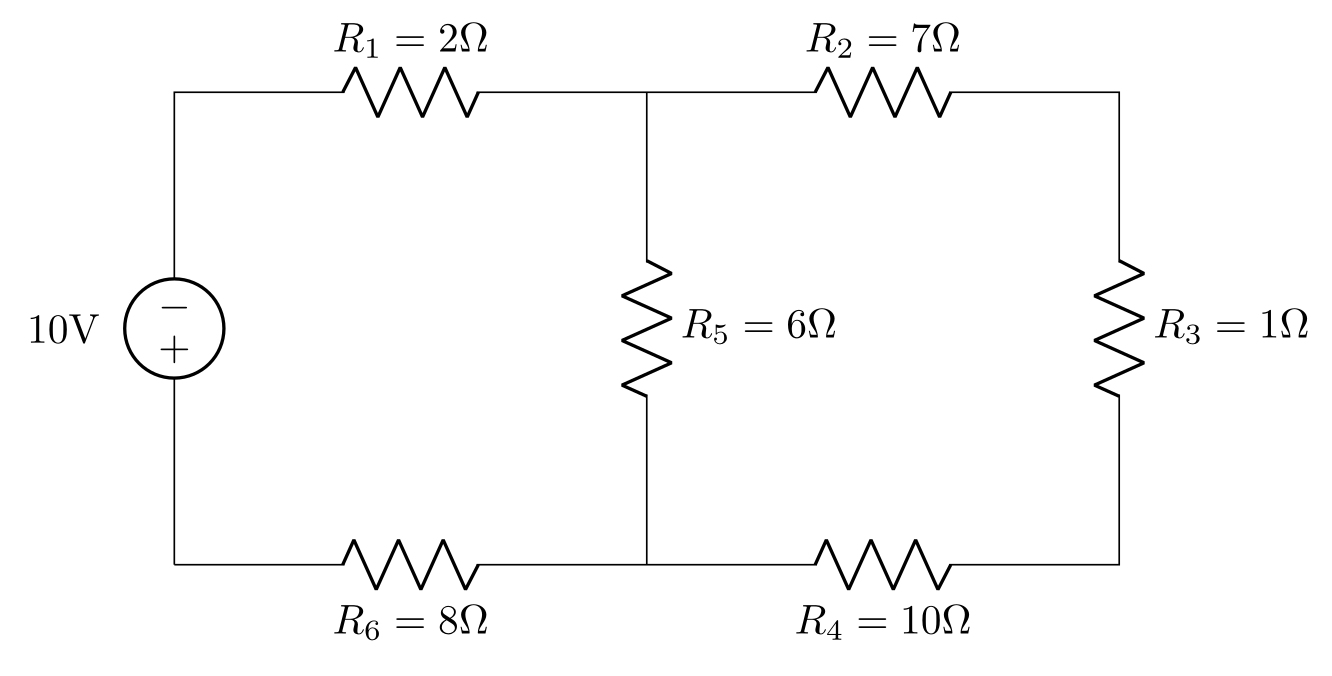
\includegraphics[scale=1.2]{Imagenes/Circuito_01.png}
\end{figure}
Revisemos primero que las resistencias $R_{2}$, $R_{3}$ y $R_{4}$ que están conectadas en serie, obtenemos una primera resistencia equivalente $R_{E1}$:
\begin{figure}[H]
\centering
\begin{circuitikz}[american voltages]
    \draw 
        (0, 0) to[V=10V] (0, 4)
        to [R, l=\mbox{$R_1=2 \Omega$}] (4, 4)
        to [R, l=\mbox{$R_2=7 \Omega$}] (8, 4)
        to [R, l=\mbox{$R_3=1 \Omega$}] (8, 0)
        to [R, l=\mbox{$R_4=10 \Omega$}] (4, 0)
        (4, 4) to [R, l=\mbox{$R_5=6 \Omega$}]  (4, 0)
        to [R, l=\mbox{$R_6=8 \Omega$}] (0, 0);
\end{circuitikz}    
\end{figure}
\begin{tikzpicture}[overlay]
    \draw [red] (8, 2) rectangle (12, 7);
\end{tikzpicture}
Entonces tendremos que:
\begin{align*}
R_{E1} = R_{2} + R_{3} + R_{4} = \SI{7}{\ohm} + \SI{1}{\ohm} + \SI{10}{\ohm} = \SI{18}{\ohm}
\end{align*}
El circuito queda como:
\begin{figure}[H]
\centering
\begin{circuitikz}[american voltages]
    \draw 
        (0, 0) to [V=10V] (0, 4)
        to [R, l=\mbox{$R_1$}] (4, 4)
        % to [R, l=\mbox{$R_2=7 \Omega$}] (8, 4)
        % to [R, l=\mbox{$R_3=1 \Omega$}] (8, 0)
        % to [R, l=\mbox{$R_4=10 \Omega$}] (4, 0)
        (4, 4) to [R, l=\mbox{$R_5$}]  (4, 0)
        to [R, l=\mbox{$R_6$}] (0, 0);
    \draw (4, 4) to[short] (6, 4)
        to [R, l=$R_{E1}$] (6, 0)
        to [short] (4, 0);
\end{circuitikz}    
\end{figure}
Se tiene que $R_{5}$ y $R_{E1}$ están conectadas en paralelo, llamamos $R_{E2}$ para resolver esas dos resistencias:
\begin{align*}
\dfrac{1}{R_{E2}} &= \dfrac{1}{R_{5}} + \dfrac{1}{R_{E1}} = \dfrac{1}{\SI{5}{\ohm}} + \dfrac{1}{\SI{18}{\ohm}}  = \dfrac{2}{9} \, \unit{\ohm} \\[1em]
R_{E2} &= \dfrac{1}{\dfrac{2}{9}} \, \unit{\ohm} = \dfrac{9}{2} \, \unit{\ohm} = \SI{4.5}{\ohm}
\end{align*}
El circuito queda con tres resistencias en serie:
\begin{figure}[H]
\centering
\begin{circuitikz}[american voltages]
    \draw 
        (0, 0) to [V=10V] (0, 4)
        to [R, l=$R_1$] (4, 4)
        to [R, l=$R_{E_2}$]  (4, 0)
        to [R, l=$R_6$] (0, 0);
\end{circuitikz}    
\end{figure}
La resistencia total del circuito es:
\begin{align*}
R_{T} = \SI{2}{\ohm} + \SI{4.5}{\ohm} + \SI{8}{\ohm} = \SI{14.5}{\ohm}
\end{align*}
El circuito se reduce a una sola resistencia, la resistencia total:
\begin{figure}[H]
\centering
\begin{circuitikz}[american voltages]
    \draw 
        (0, 0) to [V=10V] (0, 3)
        to [short] (3, 3)
        to [R, l=$R_{T}$]  (3, 0)
        to [short] (3, 0)
        to [short] (0, 0);
\end{circuitikz}    
\end{figure}
Calculamos ahora el valor de la corriente total en el circuito:
\begin{align*}
I_{T} = \dfrac{V_{T}}{R_{T}} = \dfrac{\SI{10}{\volt}}{\SI{14.5}{\ohm}} = \SI{0.689}{\ampere}
\end{align*}
Para obtener el valor de corriente y voltaje en cada resistencia, ahora hacemos un recorrido a la inversa, como $R_{T}$ corresponde a $R_{1}$, $R_{E2}$ y $R_{6}$ en serie, sabemos que el valor de corriente es el mismo en esas resistencias:
\begin{align*}
I_{1} = I_{E2} = I_{6} = \SI{0.689}{\ampere}
\end{align*}
y el voltaje en estas tres resistencias en serie, lo recuperamos con la ley de Ohm:
\begin{align*}
V_{1} &= I_{1} \, R_{1} = (\SI{0.689}{\ampere}) (\SI{2}{\ohm}) = \SI{1.378}{\volt} \\[0.5em]
V_{E2} &= I_{E2} \, R_{E2} = (\SI{0.689}{\ampere}) (\SI{4.5}{\ohm}) = \SI{3.10}{\volt} \\[0.5em]
V_{6} &= I_{6} \, R_{6} = (\SI{0.689}{\ampere}) (\SI{8}{\ohm}) = \SI{5.512}{\volt} \\[0.5em]
\end{align*}
La resistencia $R_{E2}$ corresponde a $R_{5}$ y $R_{E1}$ conectadas en paralelo, por lo que en estas dos resistencias el voltaje es el mismo:
\begin{align*}
V_{E2} = V_{5} = V_{E1} = \SI{3.10}{\volt}
\end{align*}
El valor de corriente de estas dos resistencias en paralelo, lo obtenemos con la ley de Ohm:
\begin{align*}
I_{5} &= \dfrac{V_{5}}{R_{5}} = \dfrac{\SI{3.10}{\volt}}{\SI{6}{\ohm}} = \SI{0.516}{\ampere} \\[0.5em]
I_{E1} &= \dfrac{V_{E1}}{R_{E1}} = \dfrac{\SI{3.10}{\volt}}{\SI{18}{\ohm}} = \SI{0.172}{\ampere}
\end{align*}
La resistencia $R_{E1}$ está conformada de tres resistencias en serie, por lo que la corriente en éstas será la misma:
\begin{align*}
I_{E2} = I_{2} = I_{3} = I_{4} = \SI{0.172}{\ampere}
\end{align*}
El voltaje en esas tres resistencias, lo recuperamos de la ley de Ohm:
\begin{align*}
V_{2} = I_{2} \, R_{2} = (\SI{0.172}{\ampere}) (\SI{7}{\ohm}) = \SI{1.204}{\volt} \\[0.5em]
V_{3} = I_{3} \, R_{3} = (\SI{0.172}{\ampere}) (\SI{1}{\ohm}) = \SI{0.172}{\volt} \\[0.5em]
V_{4} = I_{4} \, R_{4} = (\SI{0.172}{\ampere}) (\SI{10}{\ohm}) = \SI{1.72}{\volt} \\[0.5em]
\end{align*}
De esta manera ya hemos obtenido el valor de voltaje y corriente en cada resistencia, presentamos una tabla con los valores:
\begin{table}[H]
\centering
\renewcommand{\arraystretch}{1.1}
\begin{tabular}{| c | c | c |} \hline
Resistencia [\unit{\ohm}] & Voltaje [\unit{\volt}] & Corriente [\unit{\ampere}] \\ \hline
$R_{1} = \SI{2}{\ohm}$ & \SI{1.378}{\volt} & \SI{0.689}{\ampere} \\ \hline
$R_{2} = \SI{7}{\ohm}$ & \SI{1.204}{\volt} & \SI{0.172}{\ampere} \\ \hline
$R_{3} = \SI{1}{\ohm}$ & \SI{0.172}{\volt} & \SI{0.172}{\ampere} \\ \hline
$R_{4} = \SI{10}{\ohm}$ & \SI{1.72}{\volt} & \SI{0.172}{\ampere} \\ \hline
$R_{5} = \SI{6}{\ohm}$ & \SI{3.10}{\volt} & \SI{0.516}{\ampere} \\ \hline
$R_{6} = \SI{8}{\ohm}$ & \SI{5.512}{\volt} & \SI{0.689}{\ampere} \\ \hline
\end{tabular}
\end{table}

\end{enumerate}

\end{document}